\documentclass[10pt,handout,english]{beamer}
\usetheme{Warsaw}
\usepackage{graphicx}
\usepackage{placeins}
\usepackage{amsmath, amssymb}
\usepackage{tabu}
\usepackage{bbm}
\usepackage{booktabs}
\usepackage[round]{natbib}
\usepackage{bm}
\usepackage{ragged2e}
\usepackage{bbm}
\usepackage{hyperref}
\usepackage{amsmath}
\usepackage{xcolor}
\usepackage[super]{nth}
\hypersetup{
    colorlinks=true,
    linkcolor=blue,
    filecolor=blue,      
    urlcolor=blue,
    citecolor=black,
}

\apptocmd{\frame}{}{\justifying}{} % Allow optional arguments after frame.

\setbeamertemplate{frametitle continuation}{}

\newcommand\setItemnumber[1]{\setcounter{enumi}{\numexpr#1-1\relax}}

\DeclareMathOperator{\tr}{tr}

\newcommand{\ts}{\textsuperscript}
\newcommand{\E}{\mathbb{E}}
\newcommand{\R}{\mathbb{R}}
\newcommand{\F}{\mathcal{F}}
\newcommand{\T}{\mathbb{T}}
\newcommand{\C}{\mathbb{C}}


\newcommand{\vertiii}[1]{{\left\vert\kern-0.25ex\left\vert\kern-0.25ex\left\vert #1 
    \right\vert\kern-0.25ex\right\vert\kern-0.25ex\right\vert}}


\title[]{Bounds on $l_2$-error for hard sparse models}
\author[Kaveh S. Nobari]{Kaveh S. Nobari}
\institute[]{Lectures in High-Dimensional Statistics}
\date[27/10/2020]
{Department of Mathematics and Statistics\\ Lancaster University}
	

\begin{document}
\begin{frame}
\titlepage
\end{frame}


\begin{frame}{Contents}
\tableofcontents
\end{frame}

\section{Recap}
\frame{\tableofcontents[currentsection,currentsubsection]}

\begin{frame}[allowframebreaks]
\begin{itemize}
\setlength\itemsep{0.5em}
\item[1.] Basis pursuit problem: $\hat{\theta}=\arg \min \lVert \theta\rVert_1$, s.t. $y=X\theta^*$, where $X\in\R^{n\times d}$ and $\theta^*$ is $s$-sparse. \justifying
\item[2.] Restricted Nullspace Property: $\{\text{null}(X)\cap \{\lVert\Delta_{S^c}\rVert_1\leq \lVert\Delta_S\rVert_1\}\}=0$\justifying
\item[3.] Pairwise Incoherence (PI): $\left\lVert \frac{X'X}{n}-I \right\rVert_2\leq \delta$ \justifying
\item[4.] Restricted Isometry Property (RIP): $\vertiii{\frac{X_S'X_S}{n}- I_S}_2\leq \delta_s(X)$, where $\delta_s(X)>0$ and $\lvert S \rvert\leq s$\justifying
\item[5.] If PI holds with $\delta_s(X)<\frac{1}{3s} \rightarrow$ RN holds\justifying
\item[6.] If RIP holds with $\delta_{2s}(X)<\frac{1}{3}\rightarrow$ RN holds\justifying
\end{itemize}
\end{frame}

\section{Intuition for RIP}
\frame{\tableofcontents[currentsection,currentsubsection]}

\begin{frame}[allowframebreaks]
Our \textcolor{red}{general} aim is to solve 
\[
\hat{\theta}=\arg\min\lVert\theta\rVert_0\quad s.t.\quad y=X\theta
\]
which is hard to compute, and hence why we replace the troublesome $L_0$-norm by $L_1$-norm to obtain $\hat{\theta}$. For $\lVert\hat{\theta}\rVert_0\leq\lVert\theta^*\rVert_0\leq s$, $\lVert\Delta \rVert_0\leq 2s$, where $\Delta:=\hat{\theta}-\theta^*$.
\justifying
In order to argue that $\theta^*$ is unique , it suffices to show that $\lVert X\Delta \rVert_2^2>0$ for any at most $2s$-sparse vector $\Delta$.
\justifying
We will now show the RIP in fact implies this condition. Observe that
\[
\left\lVert\frac{X\Delta}{\sqrt{n}}\right\rVert_2^2=\frac{\Delta'X'X\Delta}{n}=\Delta'\left(\frac{X'X}{n}-I\right)\Delta+\lVert\Delta\rVert_2^2\geq -\delta\lVert\Delta\rVert_2^2+\lVert\Delta\rVert_2^2>0
\]
hold when 
\[
\vertiii{\frac{X'_SX_S}{n}- I_S}_2<1,\quad\forall \lvert S\rvert\leq 2s. 
\]
This shows that an RIP condition is sufficient for the success of the $L_0$ minimization program.
\end{frame}

\section{Estimation in noisy settings (LASSO)}
\frame{\tableofcontents[currentsection,currentsubsection]}

\begin{frame}[allowframebreaks]
Let us now turn our attention to the noisy setting, in which we observe the vector matrix pair $(y,X)\in\R^{n}\times\R^{n\times d}$ linked by the linear model
\[
y=X\theta^*+\varepsilon
\]
where $\varepsilon\in\R^n$ is the noise vector. The aim is to answer the following questions:
\begin{itemize}
\setlength\itemsep{0.5em}
\item[(a)] Can we ensure $\lVert\hat{\theta}-\theta^*\rVert_2^2$ is small?
\item[(b)] What conditions on $X$ is needed to ensure (a)?
\item[(c)] What choice of $(n,d,s)$ do we need to ensure (a)?
\end{itemize}
 A natural extension of the basis pursuit program is based on minimizing a weighted combination of the data-fidelity term $\lVert y-X\theta\rVert_2^2$ with the $L_1$-norm penalty, say of the form
\[
\hat{\theta}\in\arg\min_{\theta\in\R^d}\left\{\frac{1}{2n}\lVert y-X\theta\rVert_2^2+\lambda_n\lVert\theta\rVert_1\right\}
\] 
where $\lambda_n>0$ is a regularization parameter to be chosen by the user. What we just described, following \citet{tibshirani1996regression} is referred to as the LASSO program.

The LASSO problem can be formulated in constrained form as follows
\[
\hat{\theta}=\arg\min_{\theta\in \R^d}\left\{\frac{1}{2n}\lVert y-X\theta \rVert_2^2\right\}\quad s.t.\quad\lVert\theta\rVert_1\leq R
\]
for some radius $R>0$, or
\[
\hat{\theta}=\arg\min_{\theta\in\R^d}\lVert \theta\rVert_1\quad s.t.\quad \frac{1}{2n}\lVert y-X\theta\rVert_2^2\leq b^2
\]
for some tolerance $b>0$, where the latter form of the constrained problem is referred to as the \textcolor{red}{relaxed basis pursuit} by \citet{}. 

Looking at the regularized version of the LASSO, by the basic inequality:
\[
\frac{1}{2n}\lVert y-X\hat{\theta}\rVert_2^2+\lambda_n\lVert \hat{\theta}\rVert_1\leq \frac{1}{2n}\lVert\varepsilon\rVert_2^2+\lambda_n\lVert\theta^*\rVert_1. 
\]
Setting $\Delta:=\hat{\theta}-\theta^*$, and noting that $Y-X\hat{\theta}=\varepsilon-X\Delta$, we can expand the first 
term in the above inequality to obtain
\[
\frac{1}{2n}\lVert X\Delta\rVert_2^2-\frac{1}{n}\langle \varepsilon,X\Delta\rangle+\lambda_n\lVert\hat{\theta}\rVert_1\leq\lambda_n\lVert\theta^*\rVert_1.
\]
The goal is then to bound $\lVert\Delta\rVert_2^2$. In low dimension, a bound on $\lVert X\Delta\rVert_2^2$ would provide guarantees for $\lVert\Delta\rVert_2^2$. This is however not true in high dimension, as $X$ has a non-trivial null space.
\end{frame}

\section{Restricted eigenvalue condition}
\frame{\tableofcontents[currentsection,currentsubsection]}
\begin{frame}[allowframebreaks]
\begin{itemize}
\setlength\itemsep{0.5em}
\item Perfect recovery is no longer feasible in noisy settings. 
\justifying
\item We thus focus on bounding the $L_{2}$-error $\lVert\hat{\theta}-\theta^{*}\rVert_{2}$. 
\justifying
\item In noisy setting, the required condition is slightly stronger than the Restricted Nullspace Property - namely that the restricted eigenvalues of the matrix $\frac{X'X}{n}$ are lower bounded over a cone. In particular, for a constant $\alpha\geq1$, let us define the set
\[
\C_{\alpha}(S):=\{\Delta\in\R^{d}\mid\lVert\Delta_{S^{c}}\rVert_{1}\leq\alpha\lVert\Delta_{S}\rVert_{1}\}
\]
\justifying
\item Notice that the above set is a special case of our definition in the RNS property, which corresponds to the special case of $\alpha=1$.
\justifying
\end{itemize}
\begin{definition}[Restricted Eigenvalue condition]

The matrix X satisfies the Restricted Eigenvalue condition over $S$ with parameters $(\kappa,\alpha)$, if
\[
\frac{1}{n}\lVert X\Delta\rVert_{2}^{2}\geq\kappa\lVert\Delta\rVert_{2}^{2},\quad\forall\Delta\in\C_{\alpha}(S)
\]
\end{definition}
The Restricted Eigenvalue condition (RE hereafter) strengthens the Restricted Nullspace Property. In particular, if the RE condition holds with parameters $(\kappa,1)$ for any $\kappa>0$, then the RNS property holds. In what follows, we will prove that the error $\lVert\hat{\theta}-\theta^{*}\rVert_{2}$ in the LASSO condition is well controlled.
\end{frame}

\section{Intuition for the RE condition}
\frame{\tableofcontents[currentsection,currentsubsection]}

\begin{frame}[allowframebreaks]
In the optimisation problem
\[
\min_{\theta\in\R^{d}}\left\{ \frac{1}{2n}\lVert y-X\theta\rVert_{2}^{2}\right\} \quad\text{s.t. \ensuremath{\lVert\theta\rVert_{1}\leq R}}
\]
let us consider the radius $R=\lVert\theta^{*}\lVert_{1}$. With this setting, the true parameter vector $\theta^{*}$ is feasible for the problem. By definition, the Lasso estimate $\hat{\theta}$ minimises the quadratic cost function 
\[
L_{n}(\theta)=\frac{1}{2n}\lVert y-X\theta\rVert_{2}^{2}
\]
over the $l_{1}$-ball of radius $R$. As $n\to\infty$, it is expected that $\theta^{*}$ becomes a near-minimiser of the same cost function, so that 
\[
L_{n}(\hat{\theta})\approx L_{n}(\theta).
\]
But when does closeness in cost imply that the error vector $\Delta:=\hat{\theta}-\theta^{*}$ is small? Let us first take a look at the following image
\end{frame}
\begin{frame}
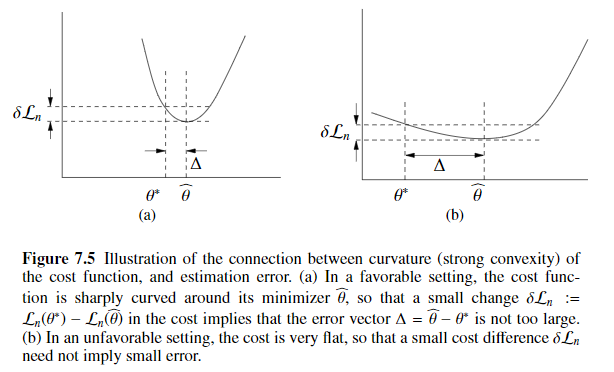
\includegraphics[width=\textwidth]{StrongConvex.png}
\end{frame}
\begin{frame}[allowframebreaks]
\begin{itemize}
\setlength\itemsep{0.5em}
\item There is a link between the cost difference of the one-dimensional function $\delta L_{n}:=L_{n}(\theta^{*})-L_{n}(\hat{\theta})$ and the error $\Delta=\hat{\theta}-\theta^{*}$ is controlled by the curvature of the cost function. 
\justifying
\item For a function in d dimensions, the curvature of a cost function is captured by the structure of its Hessian matrix $\nabla^{2}L_{n}(\theta)$, which is symmetric positive semidefinite matrix.
\justifying
\item Notice that in the special case of the quadratic cost function that underlies the LASSO 
\[
\nabla L_{n}(\theta)=\frac{1}{n}(\theta X'X-X'y)
\]
and the Hessian is calculated as 
\[
\nabla^{2}L_{n}(\theta)=\frac{1}{n}X'X
\]
\item If we could guarantee that the eigenvalues of this matrix were uniformly bounded away from zero, say that
\[
\frac{\lVert X\Delta\rVert_{2}^{2}}{n}\geq\kappa\lVert\Delta\rVert_{2}^{2}>0,\quad\forall\Delta\in\R^{d}\backslash\{0\}
\]
then we would be assured of having curvature in all directions.
\item When $d>n$ and the Hessian is a $d\times d$ with rank at most $n$, it is impossible to guarantee that it has positive curvature in all directions. 
\justifying
\item The quadratic cost function always has the below form
\end{itemize}
\end{frame}
\begin{frame}
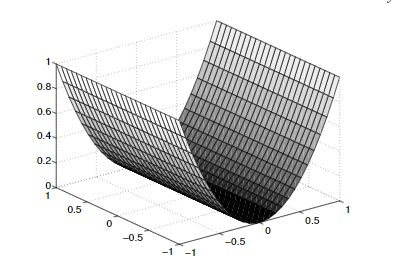
\includegraphics[width=\textwidth]{StrongConvex1.png}
\end{frame}
\begin{frame}[allowframebreaks]
\begin{itemize}
\setlength\itemsep{0.5em}
\item Although, it is curved in some directions, there is always $(d-n)$-dimensional subspace of directions in which it is completely flat, and consequently the uniform lower bound above is never satisfied. 
\justifying
\item Thus, it is necessary to relax the stringency of the uniform curvature condition and require that it holds only for a subset $\C_{\alpha}(S)$ of vectors. 
\justifying
\item If we can be assured that the subset $\C_{\alpha}(S)$ is well aligned with the curved direction of the Hessian, then a small difference in the cost function will translate into bounds on the difference between $\hat{\theta} and \theta^{*}$
\justifying
\end{itemize}
\end{frame}


\begin{frame}[allowframebreaks]
\frametitle{References}
\bibliographystyle{apa}
\bibliography{References_HDStat}
\end{frame}
\end{document}